\chapter{细胞：生命的基本单位}\label{ch:g6:cell-unit-of-life}

\Cref{ch:g5:first-look-at-cells}结尾许下了一个承诺：
那些“小房间”并不空。今年，学校的\omterm{def:g5:first-look-at-cells:microscope}{显微镜}
再次登场——玻片更好，问题也更犀利。
\omterm{def:g5:first-look-at-cells:cell}{细胞}里到底有什么？\omterm{def:g1:plants-around-us:plant}{植物}\omterm{def:g5:first-look-at-cells:cell}{细胞}与\omterm{def:g1:animals-around-us:animal}{动物}\omterm{def:g5:first-look-at-cells:cell}{细胞}有区别吗？
而\omterm{def:g5:first-look-at-cells:cell}{细胞}是生命的\emph{一部分}，还是一个\omterm{def:g5:first-look-at-cells:cell}{细胞}本身就能构成
完整的\omterm{def:g6:exploring-our-environment:components}{生物}？生物学中最小的单位
值得用一整章细致讨论。

\section{细胞内部}

\begin{definition}[细胞的组成部分]\label{def:g6:cell-unit-of-life:parts}
仔细观察可以发现，每个\omterm{def:g5:first-look-at-cells:cell}{细胞}都具有相同的基本结构：
\begin{enumerate}
  \item \emph{膜}\index{膜}，即\omterm{def:g5:first-look-at-cells:cell}{细胞}外侧薄薄的包被，
        维系\omterm{def:g5:first-look-at-cells:cell}{细胞}的完整，并
        控制物质的进出；
  \item \emph{细胞质}\index{细胞质}，即
        充满\omterm{def:g5:first-look-at-cells:cell}{细胞}内、各项工作在其中进行的胶状物质；
  \item \emph{细胞核}\index{细胞核}
        （即\cref{rem:g5:first-look-at-cells:nucleus}中的深色小点）
        是\omterm{def:g5:first-look-at-cells:cell}{细胞}的“指挥中心”，
        掌管\omterm{def:g5:first-look-at-cells:cell}{细胞}的生命活动与分裂。
\end{enumerate}
膜、\omterm{def:g5:first-look-at-cells:cell}{细胞}质与\omterm{def:g5:first-look-at-cells:cell}{细胞}核：几乎每一种\omterm{def:g1:plants-around-us:plant}{植物}、\omterm{def:g1:animals-around-us:animal}{动物}和\omterm{def:g6:decomposers-and-soil:decomposers}{真菌}的\omterm{def:g5:first-look-at-cells:cell}{细胞}
都具备的三部分基本结构。
\end{definition}

\begin{proposition}[植物细胞的额外结构]\label{prop:g6:cell-unit-of-life:plantextras}
\omterm{def:g1:plants-around-us:plant}{植物}\omterm{def:g5:first-look-at-cells:cell}{细胞}还有自己的额外结构：
\begin{itemize}
  \item 位于膜外、坚硬的\emph{细胞壁}\index{细胞壁}
——即构成洋葱表皮砖墙结构的壁，
        （见\cref{ex:g5:first-look-at-cells:classics}），
        使\omterm{def:g1:plants-around-us:plant}{植物}无需\omterm{def:g3:bones-and-muscles:skeleton}{骨骼}也能保持挺立，
        这种硬度正是\omterm{prop:g6:cell-unit-of-life:plantextras}{细胞壁}所提供的；
  \item \omterm{def:g6:cell-unit-of-life:parts}{细胞质}中含捕光物质的绿色颗粒，
——\omterm{def:g5:food-webs:roles}{生产者}的“车间”
        （见\cref{prop:g6:plants-are-producers:produce}），
        \omterm{def:g1:animals-around-us:animal}{动物}\omterm{def:g5:first-look-at-cells:cell}{细胞}中均没有；
  \item 通常还有一个充满水的大液泡，其压强
        使\omterm{def:g5:first-look-at-cells:cell}{细胞}保持饱满——\omterm{def:g1:plants-around-us:plant}{植物}萎蔫
        （见\cref{ex:g1:plants-around-us:wilt}）是
        这些液泡松弛的结果。
\end{itemize}
\end{proposition}
\admitted

\begin{omfigure}
\begin{minipage}[t]{0.48\linewidth}\centering
\begin{tikzpicture}
  \node[anchor=south west, inner sep=0] (img) at (0,0)
    {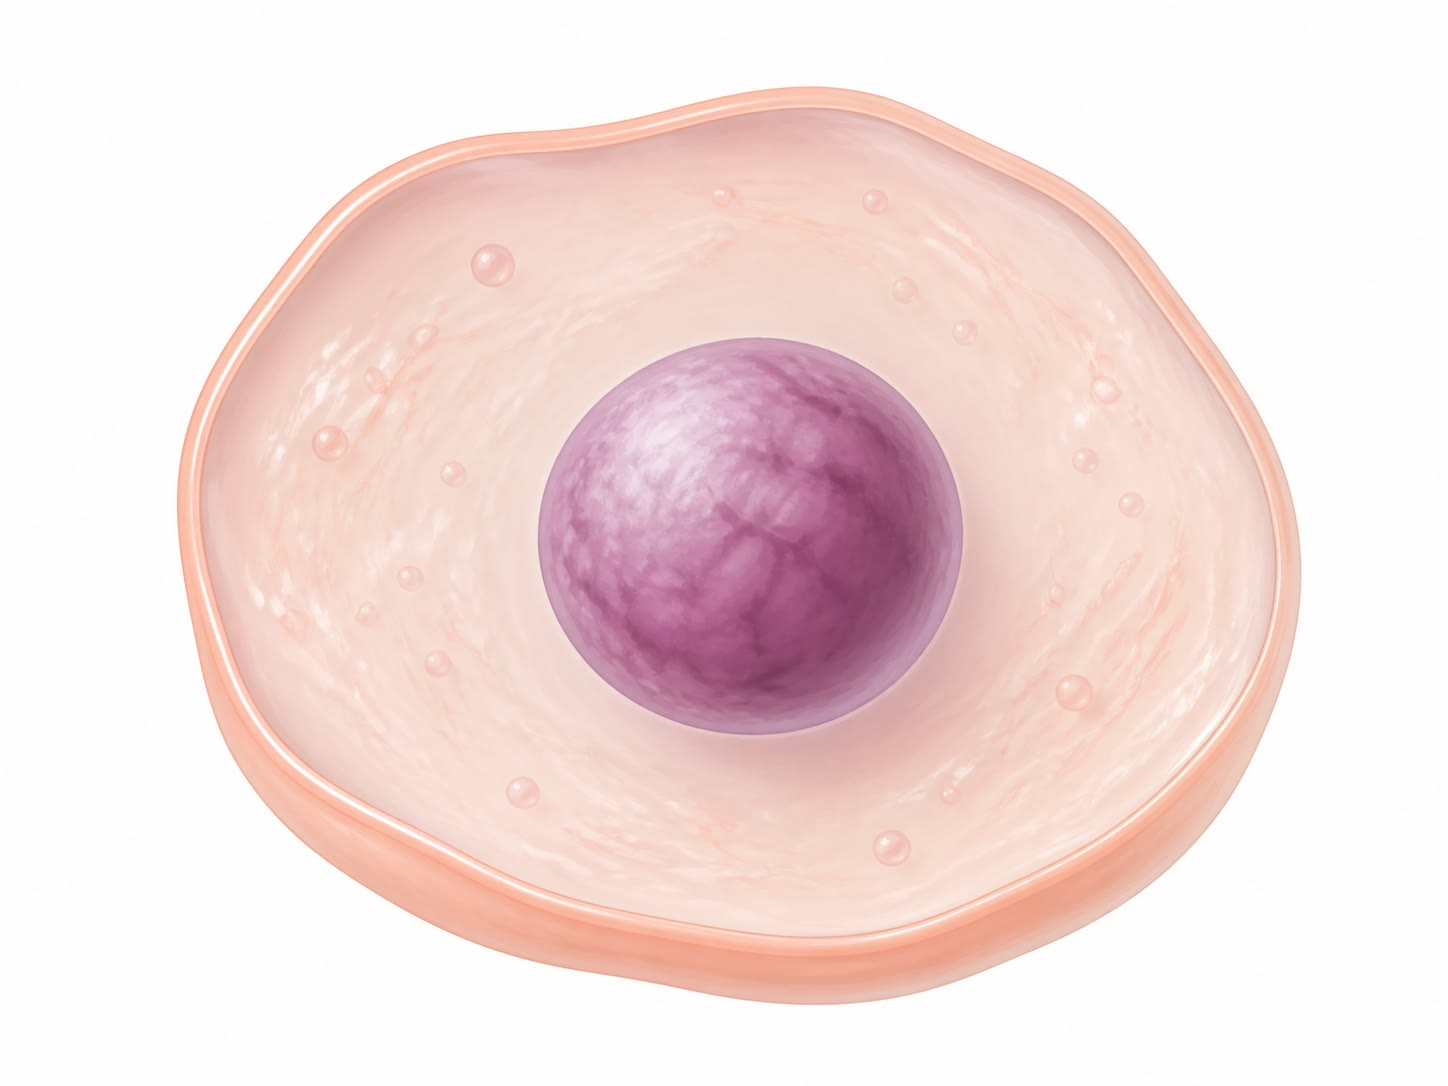
\includegraphics[width=0.9\linewidth]{images/book1/ai/fig-animal-cell.jpg}};
  \begin{scope}[x={(img.south east)}, y={(img.north west)},
      every node/.style={font=\footnotesize}]
    \draw[omDef, thick] (0.24,0.79) -- (0.12,0.93) node[above] {膜};
    \draw[omDef, thick] (0.32,0.42) -- (0.15,0.20)
      node[below] {细胞质};
    \draw[omDef, thick] (0.58,0.52) -- (0.80,0.20)
      node[below] {细胞核};
  \end{scope}
\end{tikzpicture}

{\small \omterm{def:g1:animals-around-us:animal}{动物}\omterm{def:g5:first-look-at-cells:cell}{细胞}：\\ 膜、\omterm{def:g6:cell-unit-of-life:parts}{细胞质}、\omterm{def:g6:cell-unit-of-life:parts}{细胞核}}
\end{minipage}\hfill
\begin{minipage}[t]{0.48\linewidth}\centering
\begin{tikzpicture}
  \node[anchor=south west, inner sep=0] (img) at (0,0)
    {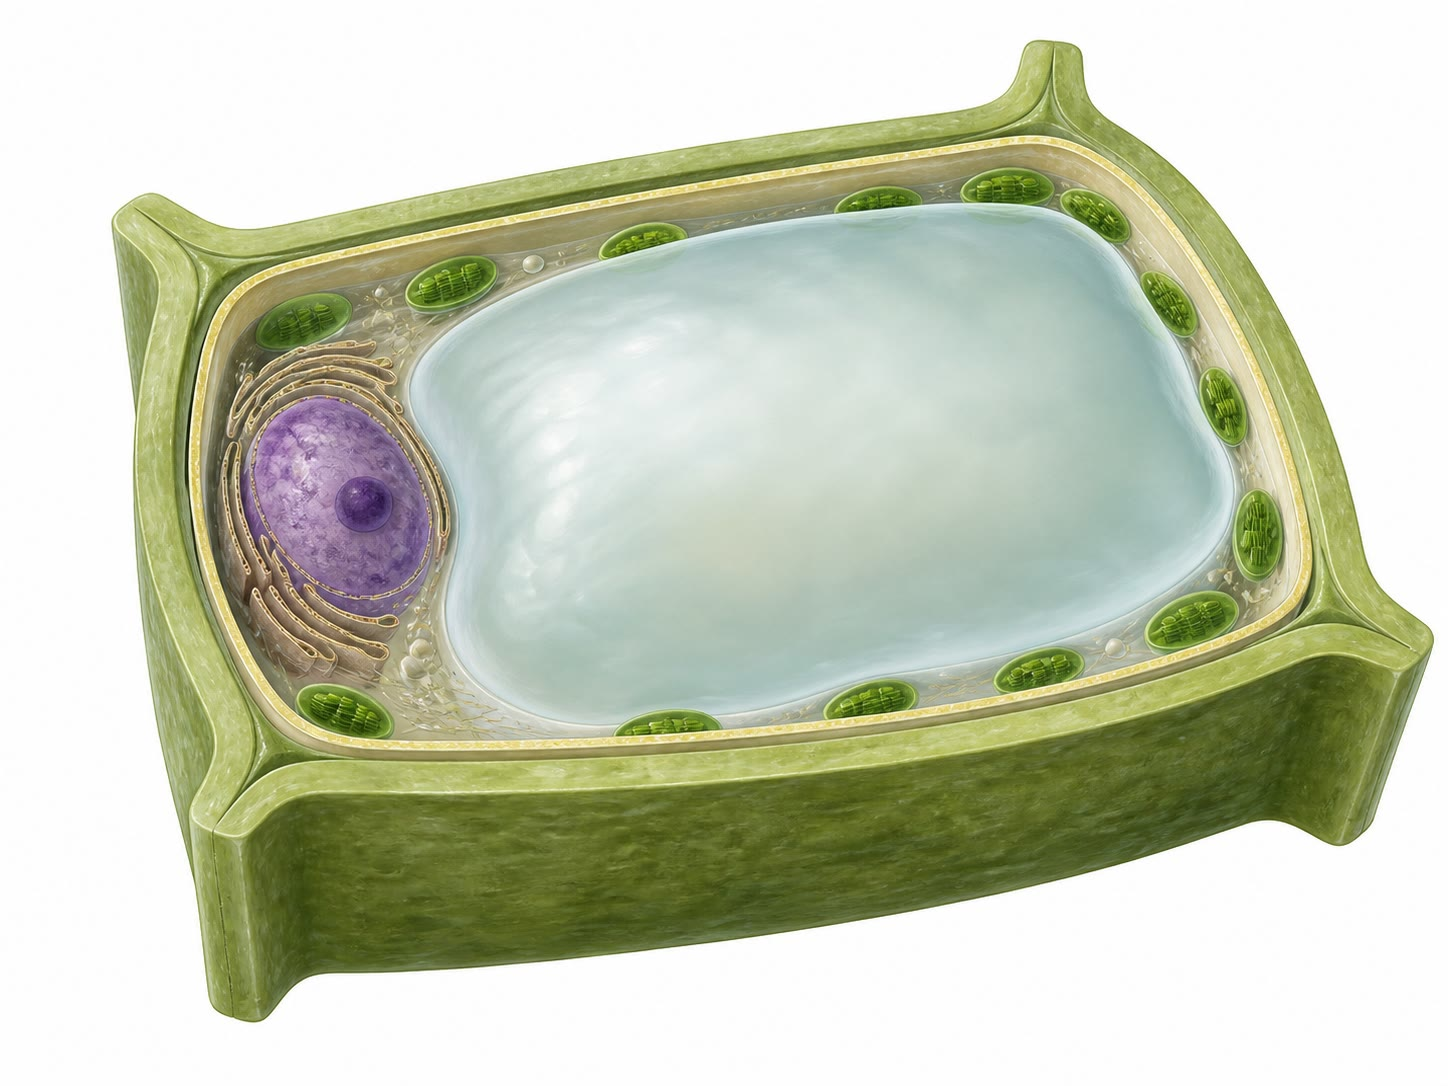
\includegraphics[width=0.98\linewidth]{images/book1/ai/fig-plant-cell.jpg}};
  \begin{scope}[x={(img.south east)}, y={(img.north west)},
      every node/.style={font=\footnotesize}]
    \draw[omMeth!60!black, thick] (0.16,0.80) -- (0.08,0.94)
      node[above] {细胞壁};
    \draw[omDef, thick] (0.26,0.53) -- (0.22,-0.04)
      node[below] {细胞核};
    \draw[omMeth!60!black, thick] (0.72,0.24) -- (0.85,-0.04)
      node[below] {绿色颗粒};
    \draw[omDef!70, thick] (0.62,0.55) -- (0.70,1.04)
      node[above] {液泡};
  \end{scope}
\end{tikzpicture}

{\small \omterm{def:g1:plants-around-us:plant}{植物}\omterm{def:g5:first-look-at-cells:cell}{细胞}：同样的结构，另加\omterm{prop:g6:cell-unit-of-life:plantextras}{细胞壁}、\\ 绿色颗粒和
液泡}
\end{minipage}

\medskip
{\small 两种经典\omterm{def:g5:first-look-at-cells:cell}{细胞}并排对照。同样的三部分结构；
\omterm{def:g1:plants-around-us:plant}{植物}\omterm{def:g5:first-look-at-cells:cell}{细胞}另有\omterm{prop:g6:cell-unit-of-life:plantextras}{细胞壁}、绿色颗粒和饱满的
液泡。}
\end{omfigure}

\begin{example}[区分两种玻片]\label{ex:g6:cell-unit-of-life:slides}
回到\omterm{def:g5:first-look-at-cells:microscope}{显微镜}前，对照
\cref{ex:g5:first-look-at-cells:classics}中的两张玻片，
现在可以为这些差异命名。洋葱表皮：壁笔直、
相交成角——即\omterm{prop:g6:cell-unit-of-life:plantextras}{细胞壁}；\omterm{def:g6:cell-unit-of-life:parts}{细胞核}被推到一侧——
是液泡的作用。口腔上皮\omterm{def:g5:first-look-at-cells:cell}{细胞}：没有\omterm{prop:g6:cell-unit-of-life:plantextras}{细胞壁}，
轮廓柔软、呈圆形——只有膜；\omterm{def:g6:cell-unit-of-life:parts}{细胞核}靠近
中央。看一眼即可判断是\omterm{def:g1:plants-around-us:plant}{植物}还是\omterm{def:g1:animals-around-us:animal}{动物}\omterm{def:g5:first-look-at-cells:cell}{细胞}。
\end{example}

\section{一个细胞中的完整生命}

\begin{definition}[单细胞生物]\label{def:g6:cell-unit-of-life:unicellular}
称\emph{单细胞}\index{单细胞}\omterm{def:g6:exploring-our-environment:components}{生物}为
由恰好一个\omterm{def:g5:first-look-at-cells:cell}{细胞}构成的完整\omterm{def:g6:exploring-our-environment:components}{生物}体
（见\cref{rem:g5:first-look-at-cells:onecelled}）。
在这层膜之内，它能取食、运动、感知并繁殖——
方式是一分为二
（即\cref{prop:g5:first-look-at-cells:growth}中的分裂，
是整个生命历程中的一环）。\omterm{ex:g6:producing-our-food:bread}{酵母}
\cref{ex:g6:producing-our-food:bread}中的\omterm{ex:g6:producing-our-food:bread}{酵母}便是一例；
任一滴池水中的游动\omterm{def:g6:exploring-our-environment:components}{生物}也是，以及大多数\omterm{def:g6:decomposers-and-soil:soil}{土壤}、
酸奶和手上的\omterm{def:g6:producing-our-food:fermentation}{微生物}。
\end{definition}

\begin{example}[一滴池水的巡游]\label{ex:g6:cell-unit-of-life:drop}
在\omterm{def:g5:first-look-at-cells:microscope}{显微镜}下观察取自水族箱绿色壁面的一滴水：
一个形如拖鞋的\omterm{def:g5:first-look-at-cells:cell}{细胞}借摆动的纤毛划水而过，速度
远超视野中的其他东西；绿色的\omterm{def:g6:cell-unit-of-life:unicellular}{单细胞}——会游动的\omterm{def:g5:food-webs:roles}{生产者}，像任何一片\omterm{def:g1:plants-around-us:parts}{叶子}那样捕获光；
一团会流动的原生质，它绕着食物流动，
把食物整个吞下。每一个都在取食、
运动、躲避，完成一整段\omterm{def:g1:animals-around-us:animal}{动物}或\omterm{def:g1:plants-around-us:plant}{植物}的生命，
全部安排在一个\omterm{def:g5:first-look-at-cells:cell}{细胞}之内。
\end{example}

\begin{remark}[一个细胞还是许多细胞：两种生存之道]\label{rem:g6:cell-unit-of-life:twoways}
\omterm{def:g6:cell-unit-of-life:unicellular}{单细胞}\omterm{def:g6:exploring-our-environment:components}{生物}用一个\omterm{def:g5:first-look-at-cells:cell}{细胞}完成全部工作；你的
身体则用数万亿个\omterm{def:g5:first-look-at-cells:cell}{细胞}完成全部工作，这些\omterm{def:g5:first-look-at-cells:cell}{细胞}
\emph{高度特化}——口腔上皮\omterm{def:g5:first-look-at-cells:cell}{细胞}用于衬里，\omterm{def:g3:bones-and-muscles:muscle}{肌肉}\omterm{def:g5:first-look-at-cells:cell}{细胞}
能够收缩（见\cref{def:g3:bones-and-muscles:muscle}），
\omterm{def:g5:brain-in-command:system}{神经}\omterm{def:g5:first-look-at-cells:cell}{细胞}负责传递
\cref{prop:g5:brain-in-command:loop}所述的信息。
多个\omterm{def:g5:first-look-at-cells:cell}{细胞}使分工成为可能；一个\omterm{def:g5:first-look-at-cells:cell}{细胞}则意味着
所有行当都挤在同一间屋子里。两种方式都行得通：\omterm{def:g6:cell-unit-of-life:unicellular}{单细胞}\omterm{def:g6:exploring-our-environment:components}{生物}是
地球上数量最多的\omterm{def:g6:exploring-our-environment:components}{生物}。
\end{remark}

\section{细胞学说}

\begin{proposition}[细胞学说]\label{prop:g6:cell-unit-of-life:theory}
两句话，凝结了数百年的探索，概括了本章
与\cref{ch:g5:first-look-at-cells}的内容：
\begin{enumerate}
  \item 一切\omterm{def:g6:exploring-our-environment:components}{生物}都由一个或多个\omterm{def:g5:first-look-at-cells:cell}{细胞}构成，
        \omterm{def:g5:first-look-at-cells:cell}{细胞}是生命的最小单位；
  \item 每个\omterm{def:g5:first-look-at-cells:cell}{细胞}都来自既有\omterm{def:g5:first-look-at-cells:cell}{细胞}的
        分裂。
\end{enumerate}
迄今从未发现例外——无论是最深的海洋，
还是最古老的岩石水洼，第二句话有一个深远的推论：
今天存活的每个\omterm{def:g5:first-look-at-cells:cell}{细胞}，都延续着一条可追溯到最早生命的
从未中断的分裂链条——这是
\omterm{prop:g6:classification-kinship:kinship}{亲缘关系}（见\cref{prop:g6:classification-kinship:kinship}），
在\omterm{def:g5:first-look-at-cells:cell}{细胞}尺度上的书写。
\end{proposition}
\admitted

\begin{method}[在细胞尺度上读懂任何生物]\label{met:g6:cell-unit-of-life:read}
面对任何\omterm{def:g6:exploring-our-environment:components}{生物}时：
\begin{enumerate}
  \item 先问：一个\omterm{def:g5:first-look-at-cells:cell}{细胞}，还是许多\omterm{def:g5:first-look-at-cells:cell}{细胞}？
  \item 若是许多\omterm{def:g5:first-look-at-cells:cell}{细胞}，预期会有各种特化类型——衬里的、
        运输的、收缩的、指挥的；
  \item 是\omterm{def:g1:plants-around-us:plant}{植物}还是\omterm{def:g1:animals-around-us:animal}{动物}？看看有无\omterm{prop:g6:cell-unit-of-life:plantextras}{细胞壁}和绿色颗粒，
        在\omterm{def:g5:first-look-at-cells:microscope}{显微镜}下观察；
  \item 凡是观察到的生长、修复或繁殖，
        都要转化为\omterm{def:g5:first-look-at-cells:cell}{细胞}的分裂——第二句
        保证这种转化必然存在。
\end{enumerate}
\end{method}

\begin{example}[本书中的细胞学说]\label{ex:g6:cell-unit-of-life:atwork}
第一句话支撑了\omterm{prop:g5:first-look-at-cells:principle}{生命的统一性}
（见\cref{prop:g5:first-look-at-cells:principle}）；第二句话支撑了
分裂式生长
（见\cref{ex:g5:first-look-at-cells:one}），面团中\omterm{ex:g6:producing-our-food:bread}{酵母}的倍增、
温暖堆肥中\omterm{def:g6:decomposers-and-soil:decomposers}{分解者}的繁殖，
以及
\cref{ch:g6:producing-our-food}中的\omterm{def:g6:producing-our-food:fermentation}{微生物}劳动。一个简单的学说，承载着
本学年生物学的大部分内容。
\end{example}

\section{练习}

\begin{exercise}[$\star$]\label{exo:g6:cell-unit-of-life:1}
说出每个\omterm{def:g5:first-look-at-cells:cell}{细胞}的三部分结构，
并说明各部分的作用。
\end{exercise}

\begin{exercise}[$\star$]\label{exo:g6:cell-unit-of-life:2}
说出\omterm{def:g1:plants-around-us:plant}{植物}\omterm{def:g5:first-look-at-cells:cell}{细胞}特有的三种结构，并说明各自的作用。
\end{exercise}

\begin{exercise}[$\star$]\label{exo:g6:cell-unit-of-life:3}
在\omterm{def:g5:first-look-at-cells:microscope}{显微镜}下，如何区分洋葱表皮\omterm{def:g5:first-look-at-cells:cell}{细胞}和
口腔上皮\omterm{def:g5:first-look-at-cells:cell}{细胞}？列出两个可见的差异。
\end{exercise}

\begin{exercise}[$\star$]\label{exo:g6:cell-unit-of-life:4}
什么是\omterm{def:g6:cell-unit-of-life:unicellular}{单细胞}\omterm{def:g6:exploring-our-environment:components}{生物}？请说出
本章中的两种。
\end{exercise}

\begin{exercise}[$\star$]\label{exo:g6:cell-unit-of-life:5}
陈述\omterm{def:g5:first-look-at-cells:cell}{细胞}学说的两句话。
\end{exercise}

\begin{exercise}[$\star$]\label{exo:g6:cell-unit-of-life:6}
\omterm{def:g6:cell-unit-of-life:unicellular}{单细胞}\omterm{def:g6:exploring-our-environment:components}{生物}如何繁殖？
\end{exercise}

\begin{exercise}[$\star\star$]\label{exo:g6:cell-unit-of-life:7}
为什么\omterm{def:g1:plants-around-us:plant}{植物}没有\omterm{def:g3:bones-and-muscles:skeleton}{骨骼}也能直立？哪两种\omterm{def:g1:plants-around-us:plant}{植物}\omterm{def:g5:first-look-at-cells:cell}{细胞}结构
共同承担这一功能——从\omterm{def:g5:first-look-at-cells:cell}{细胞}尺度看，
萎蔫是怎么回事？
\end{exercise}

\begin{exercise}[$\star\star$]\label{exo:g6:cell-unit-of-life:8}
哪种\omterm{def:g5:first-look-at-cells:cell}{细胞}结构是\omterm{def:g5:food-webs:roles}{生产者}的“车间”（见
\cref{prop:g6:plants-are-producers:produce}）？根据
\cref{prop:g6:matter-from-food:transform}，为什么
每个\omterm{def:g1:animals-around-us:animal}{动物}\omterm{def:g5:first-look-at-cells:cell}{细胞}都必须缺少它？
\end{exercise}

\begin{exercise}[$\star\star$]\label{exo:g6:cell-unit-of-life:9}
依据\cref{rem:g6:cell-unit-of-life:twoways}，找出你身体的
三种特化\omterm{def:g5:first-look-at-cells:cell}{细胞}，并说明每种\omterm{def:g5:first-look-at-cells:cell}{细胞}的分工。
\end{exercise}

\begin{exercise}[$\star\star$]\label{exo:g6:cell-unit-of-life:10}
依据
\cref{met:g6:cell-unit-of-life:read}，用\omterm{def:g5:first-look-at-cells:cell}{细胞}分裂来解释下列情形：伤口愈合；
面团一夜间体积翻倍；一条正在生长的\omterm{ex:g2:animals-grow-up:frog}{蝌蚪}。
\end{exercise}

\begin{exercise}[$\star\star$]\label{exo:g6:cell-unit-of-life:11}
一滴池塘水中的绿色游动者，是能够捕获光的\omterm{def:g6:cell-unit-of-life:unicellular}{单细胞}
  \omterm{def:g6:exploring-our-environment:components}{生物}。它们承担的是
\cref{def:g5:food-webs:roles}中的哪种分工？这使它们在
池塘\omterm{def:g5:food-webs:web}{食物网}中成为什么？
\end{exercise}

\begin{exercise}[$\star\star\star$]\label{exo:g6:cell-unit-of-life:12}
认真对待\omterm{def:g5:first-look-at-cells:cell}{细胞}学说的第二句话，正如
\cref{rem:g6:classification-kinship:implies}对待那棵树那样：
你的某个口腔\omterm{def:g5:first-look-at-cells:cell}{细胞}，与遥远的过去之间
由怎样一条不曾中断的链条相连？请用一句话
陈述由此得出的结论。
\end{exercise}

\section{问题：显微镜下的下午}

\begin{problem}[{周末问题——四张玻片，一个学说
学说}]\label{pb:g6:cell-unit-of-life:1}
班级的\omterm{def:g5:first-look-at-cells:microscope}{显微镜}下午活动：四个站点，四张
玻片——洋葱表皮（A）、口腔刮片（B）、一滴
池塘水（C）、酸奶涂片（D）。每组依次参观
全部四个站点，并留存绘图。

\medskip\noindent\textbf{第一部分——站点 A 和 B。}
\begin{enumerate}
  \item 在站点 A，小组画出的是壁笔直的
        “方砖”，每块都有一个深色斑点被挤向一侧。
        请指出\omterm{prop:g6:cell-unit-of-life:plantextras}{细胞壁}、斑点，以及造成拥挤的
        那个“元凶”。
  \item 站点 B：\omterm{def:g5:first-look-at-cells:cell}{细胞}呈圆形，没有\omterm{prop:g6:cell-unit-of-life:plantextras}{细胞壁}，斑点
        位于中央。列出 A 中\omterm{def:g5:first-look-at-cells:cell}{细胞}所具有、而 B 中\omterm{def:g5:first-look-at-cells:cell}{细胞}
        所缺少的结构，以及两者共有的结构。
  \item 一位队友问，取自地下生长\omterm{ex:g4:plants-without-seeds:bulbtuber}{鳞茎}的洋葱\omterm{def:g5:first-look-at-cells:cell}{细胞}为何
        看不到绿色颗粒。请
        结合颗粒的功能与\omterm{ex:g4:plants-without-seeds:bulbtuber}{鳞茎}的生长位置作答。
  \item 玻片 B 上的是谁的\omterm{def:g5:first-look-at-cells:cell}{细胞}？请说明
        这对\omterm{def:g5:first-look-at-cells:cell}{细胞}学说第二句意味着什么：每个
        \omterm{def:g5:first-look-at-cells:cell}{细胞}分别从何而来？
\end{enumerate}

\medskip\noindent\textbf{第二部分——站点 C 和 D。}
\begin{enumerate}[resume]
  \item 站点 C：形如拖鞋的“划桨者”、绿色游动者、
        流动的“团块”。对每一个，请说出
        一分钟观察中可见的生命活动
——并判断每一个各是什么。
  \item 绿色游动者是\omterm{def:g6:cell-unit-of-life:unicellular}{单细胞}，却
        属于\omterm{def:g5:food-webs:roles}{生产者}。绘图中必须画出哪一种结构，
        才能证明这一点？
  \item 站点 D 的酸奶涂片中，可见大量成对或成链排列的微小
        \omterm{def:g5:first-look-at-cells:cell}{细胞}。请将它们与
        \cref{ex:g6:producing-our-food:yogurt}相联系：这些\omterm{def:g5:first-look-at-cells:cell}{细胞}
        对牛奶做了什么？它们在本章的术语中是
        什么？
  \item 有一组声称玻片 D 上显示的是“没有\omterm{def:g6:exploring-our-environment:components}{生物}，只有
        斑点”。哪一项单一观察
——只要耐心等待或将玻片保温——就能
        判定这些斑点是否有生命，
        依据\omterm{def:g5:first-look-at-cells:cell}{细胞}学说第二句？
\end{enumerate}

\medskip\noindent\textbf{第三部分——撰写报告。}
\begin{enumerate}[resume]
  \item 报告须按以下\omterm{def:g3:sorting-living-things:criterion}{标准}对四张玻片进行分类：\omterm{def:g5:first-look-at-cells:cell}{细胞}是
        单个还是多个？属于\omterm{def:g1:plants-around-us:plant}{植物}、\omterm{def:g1:animals-around-us:animal}{动物}，还是都不是？请完成分类。
  \item 下午的每幅绘图都显示出相同的
        三部分结构组合。请写出这一组合，
        并说明这种普遍性为
        \cref{prop:g5:first-look-at-cells:principle}提供了证据。
  \item 老师总结道：“你们今天画下的每一样东西，
        都曾经只是一个\omterm{def:g5:first-look-at-cells:cell}{细胞}。”请为这句话辩护，
        分别针对洋葱、口腔\omterm{def:g5:first-look-at-cells:cell}{细胞}的提供者
        以及酸奶中的\omterm{def:g5:first-look-at-cells:cell}{细胞}链。
  \item 将下午的发现表述为\omterm{def:g5:first-look-at-cells:cell}{细胞}学说
——两句话——并为每张玻片标出
        它最能说明的是哪一句。
\end{enumerate}
\end{problem}
